{\let\clearpage\relax \chapter{Foundations}\label{ch:foundations}}
In this chapter, we introduce the SQW, a tool designed to generate literature search queries for evaluation in later stages of the project. We begin by outlining the required inputs for the tool, clarifying how users interact with it. Then, we provide an overview of the two main stages of the SQW, explaining the methodology and rationale behind its design.

We also review related work in the field, focusing on approaches that evaluate literature search queries. We assess the strengths and limitations of these methods and discuss how the queries they generate are evaluated using existing datasets. This review provides essential context for understanding the current landscape of literature query evaluation research, which, to our knowledge, has gaps in the area of automatic evaluation. While existing work offers valuable insights into specific aspects of query evaluation, it often overlooks the variety of factors influencing query performance across diverse datasets and domains. This gap highlights the need for further exploration into more robust and automated evaluation frameworks.

\section{Search Query Writer}\label{sec:sqw}
The SQW is a tool based on an LLM, specifically using GPT-4o, to systematically generate literature search queries. The only required input for this tool, which is the main focus of this work, is the \textbf{Topic}. Users are required to provide a topic for generating a search query, irrespective of the scientific field—for example, \textit{Synthetic Biology}. 

Several optional inputs are available to enhance the quality of the generated query, including:
\begin{itemize}
	
\item \textbf{Negative Keywords:} Terms that should be excluded to avoid unwanted results.
\item \textbf{Description:} A description that serves as an alignment mechanism to clarify the task’s intent.
\item \textbf{Modes:} Three selectable modes (Strict, Moderate, Creative) that control the temperature of the LLM to manage the level of randomness in responses.
\item \textbf{Depth:} A parameter that specifies how comprehensively the topic should be analyzed.
\item \textbf{Supporting Documents:} Users can upload a PDF, ideally a survey or overview document on the topic, which helps the tool acquire knowledge about the scientific field and better align with the research intent.

\end{itemize}
These additional inputs are intended to refine and tailor the search query to more closely match the user's research goals, but will not be extensively tested in this work.

To generate a literature search query, we designed the SQW to take a human-like approach, divided into two main steps: \textbf{Knowledge Enrichment} and \textbf{Iterative Scientific Fine-Tuning}.

The objective of the \textbf{Knowledge Enrichment} step is to provide the LLM with contextual information about the research topic. This is achieved by first retrieving information from Wikipedia based on the given topic. Specifically, the first 4,000 characters from the top-\( k \) pages are collected and summarized before being passed into the LLM's memory. ArXiv is queried in a similar manner to gather relevant research content. Additionally, we perform an online search using DuckDuckGo\footnote{\url{https://duckduckgo.com/}}, aggregating results to offer a broader understanding of the topic.

\begin{figure}[!h]
	\centering
	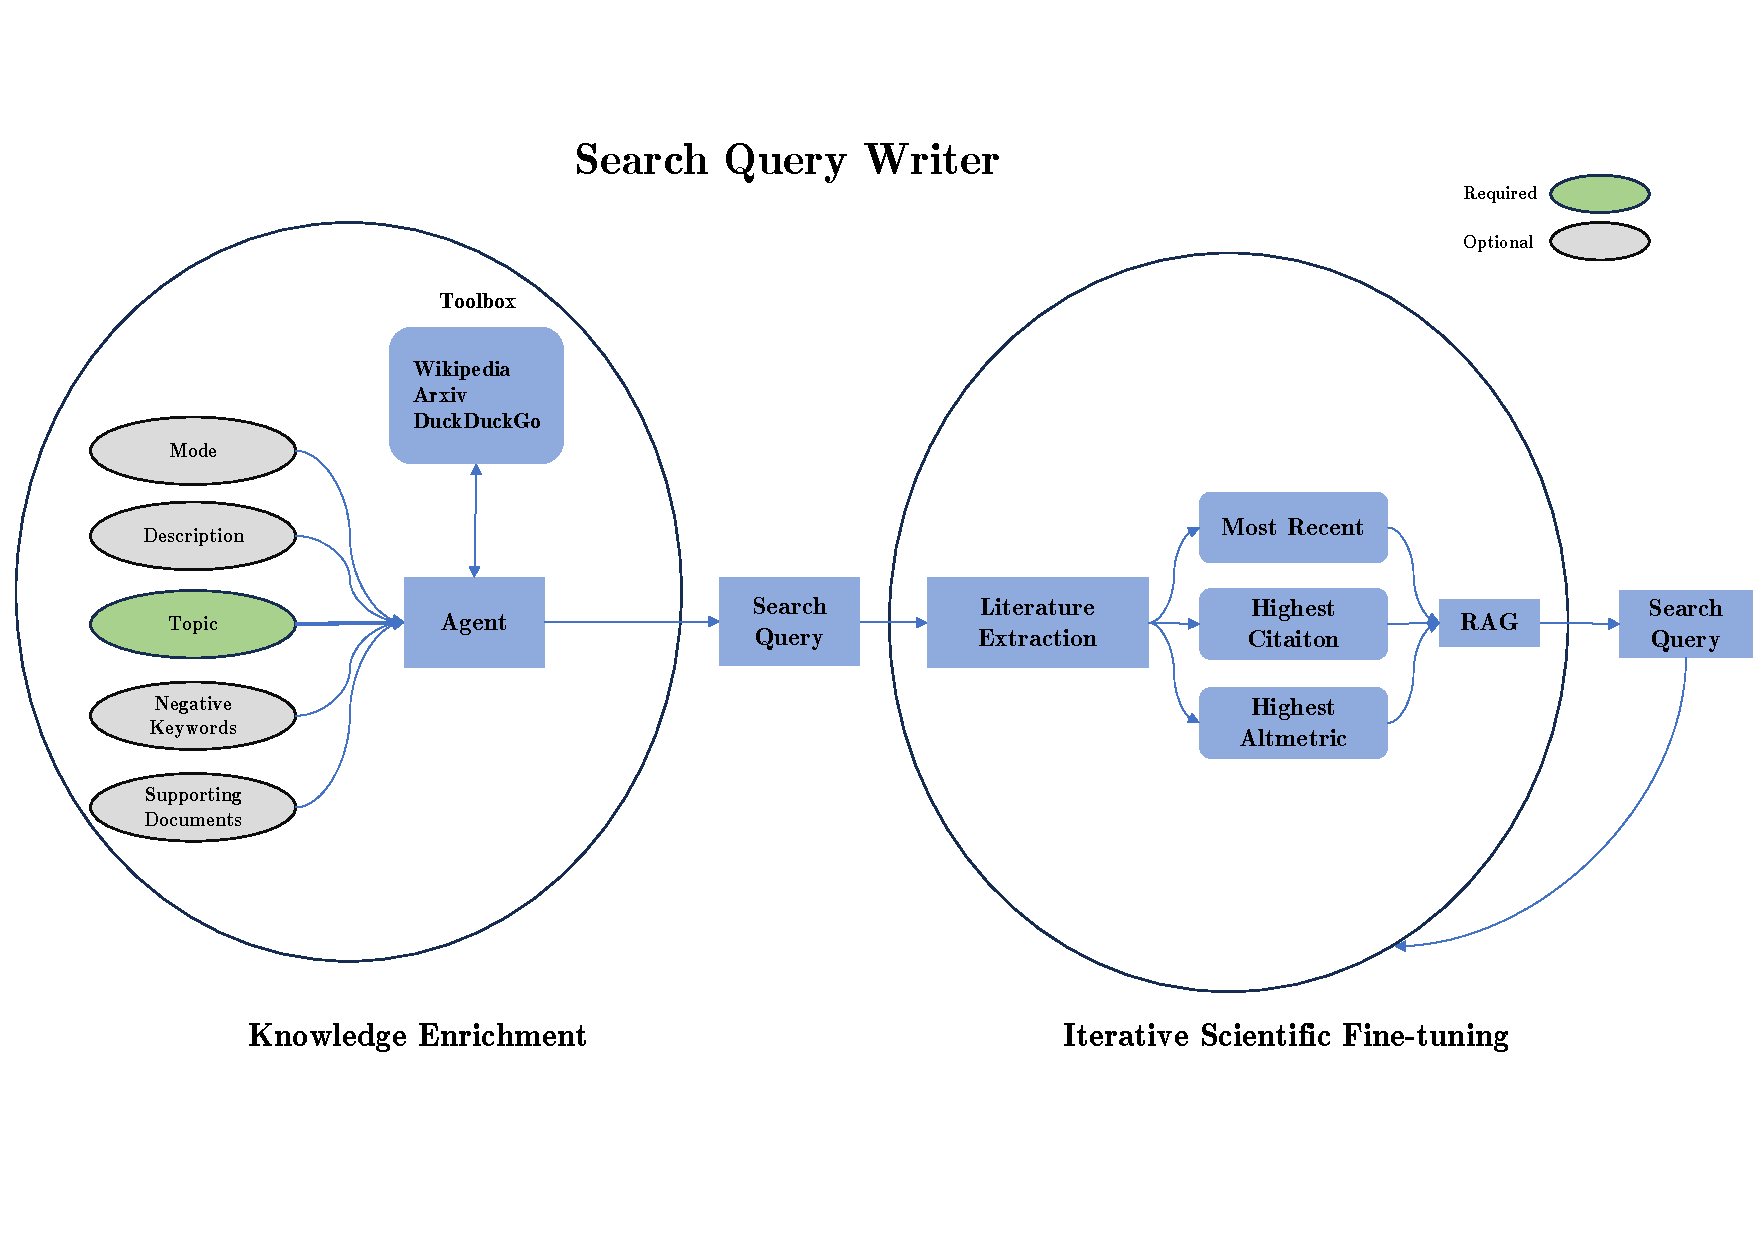
\includegraphics[scale=.48]{pics/sqw-overview.pdf}
	\caption[Search Query Writer]{A simplified overview of the SQW. The process begins with the Knowledge Enrichment stage, where the model receives input data and sends it to an LLM agent equipped with a suite of tools to gain insights into the topic. Based on this understanding, the model generates a well-structured search query, formatted and executed across multiple dimensions to retrieve a relevant selection of literature. Within this literature set, RAG is applied to identify the most pertinent keywords, which are compiled into an optimized search query. This query can be iteratively refined to enhance overall search quality.}
	\label{fig:sqw-overview}
\end{figure}

To reduce Recency bias \autocite{Deldjoo2024}, which refers to the tendency of the attention mechanism to favor more recent information, each of the steps is conducted in a separate API session, with results stored independently for future use. This approach ensures a that the LLM is biased towards the recently fetched results from prior steps.

The output of this first stage is a list of keywords, typically presented in a transfer-list format, as shown in \autoref{fig:sqw-stage1}. This transfer-list contains two categories: specific and general keywords, along with additional information such as the number of publications found per keyword. The primary goal of this step is to enable the user to assess the relevance of each keyword. If a keyword is deemed too broad, it should be moved to the general list; if it accurately targets the specified topic, it should remain in the specific list. Additionally, the user is required to provide an overarching topic that limits the scope of the general keywords to align more closely with the research intent. The output of this stage will be the queries used for the final evaluation.

\begin{figure}
	\centering
	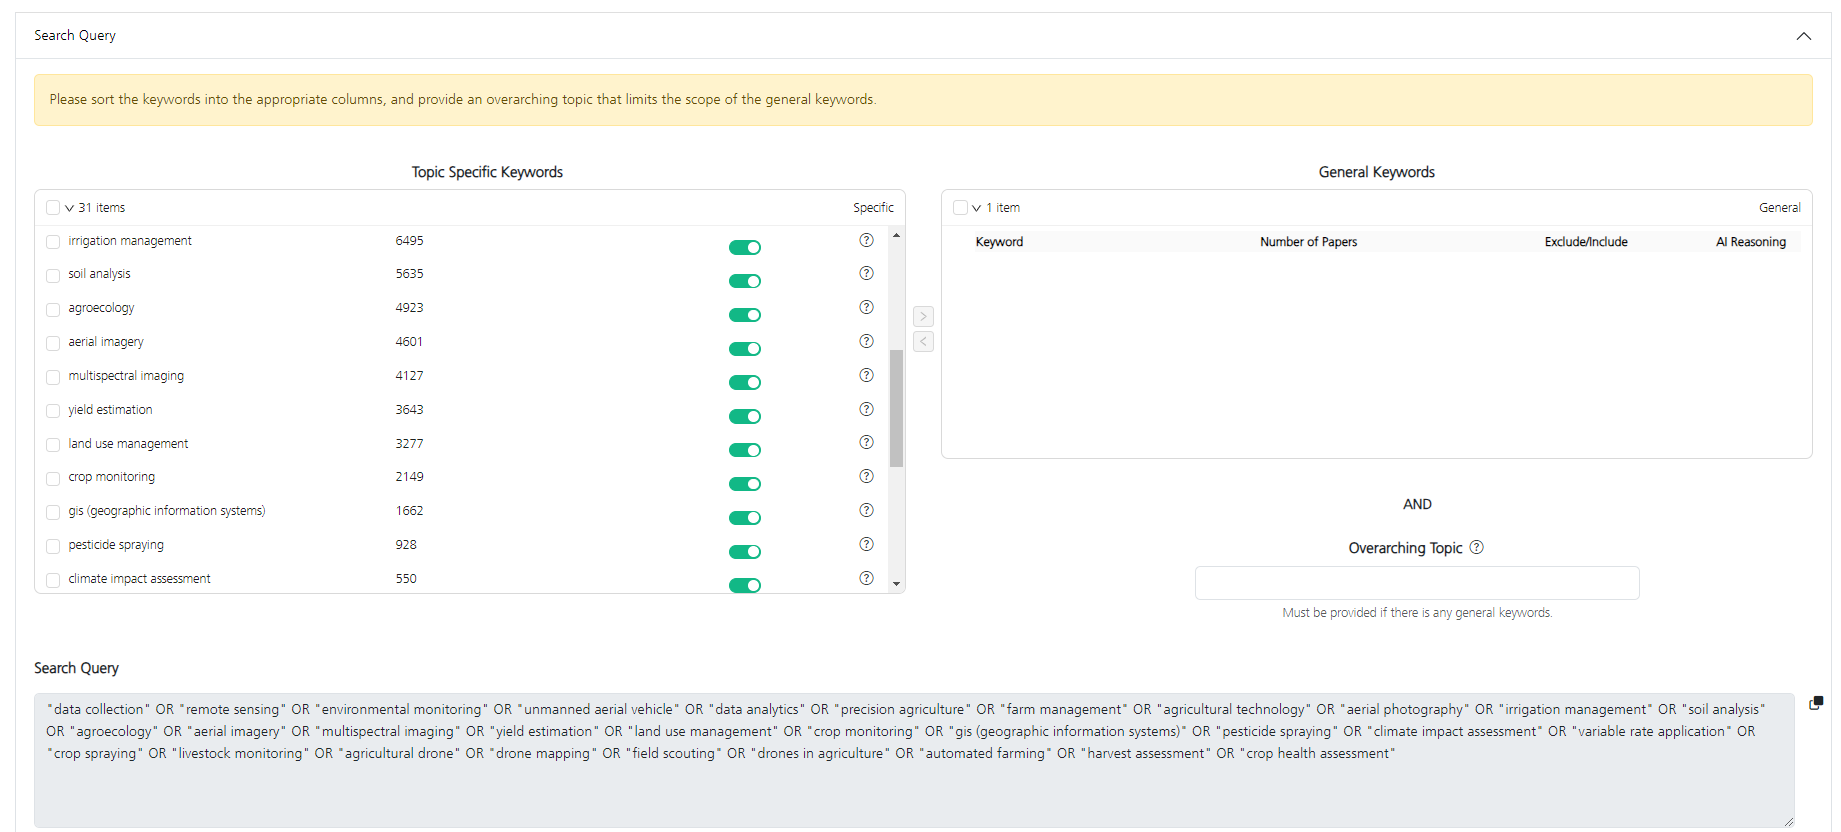
\includegraphics[height=200px, width=400px]{pics/sqw-stage1.png}
	\caption[SQW Knowledge Enrichment]{A screenshot of the SQW UI after completing the Knowledge Enrichment stage. On the left, a list of keywords is displayed alongside the number of publications associated with each keyword when used as a search term. The keywords on the right-hand side were manually categorized as general and can be roughly assessed by the number of associated publications. To narrow the scope of general keywords, we selected "agriculture" as the overarching topic. The final generated query is displayed and updated interactively as values in the transfer lists are adjusted.}
	\label{fig:sqw-stage1}
\end{figure}


The \textbf{iterative scientific fine-tuning} on the other hand approaches more scientific sources, namely dimensions.ai, which is a literature database that offers quick access to publications across a wide range of journals. The query generated in the earlier stage is then used to prompt dimensions three times, once to retrieve the most cited 1k literature, a second time to retrieve the newest 1k literature, and one last 1k to retrieve the most relevant literature based on their altmetric rating. The results are then combined, and duplicates are removed, yielding a set of publications. For this set, the titles and abstracts are extracted and processed using OpenAI's embedding model. Finally, a simple RAG pipeline is applied to retrieve publications which are then used to generate relevant keywords based on their content.

\section{Related Work}\label{sec:relwork}

SLRs are widely used across various fields, allowing researchers to conduct a comprehensive manual review of scientific topics and identify publications that answer a set of research questions. However, one significant challenge with this approach has been the exponential growth in the number of publications, which makes conducting unbiased reviews increasingly difficult. In the age of technological advancements, we can now use these technologies such as LLMs, Topic Modeling, Semantic Embeddings and much more to assist in investigating topics without the need to manually sift through extensive lists of potentially irrelevant publications. To address this issue, a series of works have been proposed within the Conference and Labs of the Evaluation Forum (CLEF) \autocite{kanoulas2017clef, kanoulas2018clef, kanoulas2019clef}. These works focus on the evaluation of empirical medical research, utilizing a dataset of medical literature. They introduce two primary tasks: Task 1, which involves identifying relevant studies from the PubMed medical database, and Task 2, which assesses the ranking of studies following title and abstract screening. Notably, the evaluation pipeline, along with the dataset and descriptions of these tasks, are publicly accessible on GitHub\footnote{\url{https://github.com/CLEF-TAR/tar/tree/master}}.

LLMs have had significant impact on modern technology, including in scientific research, where they have provided remarkable improvements in efficiency. While the processing efficiency of LLMs is unprecedented, the quality of their output in various domains is still being explored. The work by Wang \autocite{wang2023can} investigated the performance of ChatGPT in generating Boolean search queries for literature reviews. Specifically, it evaluated the effectiveness of ChatGPT in constructing queries for SLRs using different prompting techniques, including zero-shot, few-shot and iterative guided approaches. The evaluation used the CLEF datasets \autocite{kanoulas2017clef, kanoulas2018clef, kanoulas2019clef} and an additional medical dataset containing a collection of seeds \autocite{Wang_2022}. Although the results highlight the limitations of ChatGPT's performance, this work underscores the potential of LLMs to aid literature review, especially when supported by examples or more advanced, structured pipelines.

A broader and more diverse evaluation of the quality of automatically generated literature search queries for SLRs was conducted by Badami \autocite{badami2023adaptive}. In this work, they introduced a pipeline that generates literature search queries based on a given research question and abstracts from previously identified relevant publications. The evaluation was performed against a dataset they constructed, which contains the results of 10 SLRs, including candidate papers, queries used, and relevant papers identified in each review. For example, in the review $SLR_1$, a total of 7,002 candidate papers were retrieved using search query $S$, from which a subset of 59 relevant papers $RP$ was identified. To assess their proposed approach, they compared the generated queries in various settings using recall and precision metrics, benchmarking them against the original search query $S$. The dataset is publicly available on Zenodo\footnote{\url{https://tinyurl.com/496zuar3}}.
